%% This is file `elsarticle-template-1-num.tex',
%%
%% Copyright 2009 Elsevier Ltd
%%
%% This file is part of the 'Elsarticle Bundle'.
%% ---------------------------------------------
%%
%% It may be distributed under the conditions of the LaTeX Project Public
%% License, either version 1.2 of this license or (at your option) any
%% later version.  The latest version of this license is in
%%    http://www.latex-project.org/lppl.txt
%% and version 1.2 or later is part of all distributions of LaTeX
%% version 1999/12/01 or later.
%%
%% Template article for Elsevier's document class `elsarticle'
%% with numbered style bibliographic references
%%
%% $Id: elsarticle-template-1-num.tex 149 2009-10-08 05:01:15Z rishi $
%% $URL: http://lenova.river-valley.com/svn/elsbst/trunk/elsarticle-template-1-num.tex $
%%
\documentclass[preprint,review,times,12pt]{elsarticle}

%% Use the option review to obtain double line spacing
%% \documentclass[preprint,review,12pt]{elsarticle}

%% Use the options 1p,twocolumn; 3p; 3p,twocolumn; 5p; or 5p,twocolumn
%% for a journal layout:
%% \documentclass[final,1p,times]{elsarticle}
%% \documentclass[final,1p,times,twocolumn]{elsarticle}
%% \documentclass[final,3p,times]{elsarticle}
%% \documentclass[final,3p,times,twocolumn]{elsarticle}
%% \documentclass[final,5p,times]{elsarticle}
%% \documentclass[final,5p,times,twocolumn]{elsarticle}


\usepackage[left=1in, right=1in, top=1in, bottom=1in]{geometry}
\usepackage{graphicx}
\usepackage{amssymb}
\usepackage{amsthm}
\usepackage{amsmath}
\usepackage{lineno}
\usepackage{caption}
\usepackage{natbib}

\journal{Ecological Modelling}
\setcitestyle{authoryear,round,semicolon,sort}
\bibliographystyle{apalike}
\begin{document}
\begin{frontmatter}

\title{The performance of presence-based and process-based species distribution models}

\author[NREN,CS]{Tim M. Szewczyk}
\author[CS]{Marek Petrik}
\author[NREN]{Jenica M. Allen}

\address[NREN]{Department of Natural Resources and the Environment, University of New Hampshire}
\address[CS]{Department of Computer Science, University of New Hampshire}

\begin{abstract}
Abstract here
\end{abstract}

\begin{keyword}
keywords
\end{keyword}

\end{frontmatter}
\linenumbers



\section{Introduction}
\label{S:1}
% SDMs and the prevalence of occurrenc-based methods (And)
1. General introduction about species distribution models and the historical prevalence of occurrence-based SDMs.

% Process-based SDMs as an alternative, including a specific example or two (But)
2. The rise of process-based SDMs (or at least the rise in advocacy for process-based SDMs), including some specific examples of their use, since that was the main question raised at ISEM.  

% Expected benefits of process-based SDMs (And)
3. Expected benefits of process-based SDMs

% Benefits of occurrence-based, and the unknowns of process-based performance (But) 
4. Potential downsides of process-based SDMs

% Mission statement (Therefore)
We evaluate the performance of an occurrence-based SDM and three process-based SDMs for two virtual species. We investigate the ability of each SDM  to predict the true distributions under ideal conditions, as well as under various realistic data and modelling scenarios. Specifically, we ask: 1) Do process-based models outperform MaxEnt overall? 2) are process-based or occurrence-based SDMs more susceptible to particular data deficiencies? And 3) do common modelling errors negate any improved performance observed in the process-based SDMs?




\section{Methods}
% General outline of the process (?)
% Range boundary definitions
% Virtual species simulation
% Virtual ecologist simulation
% SDM methods we compared

\label{S:2}
\begin{figure}
	\centering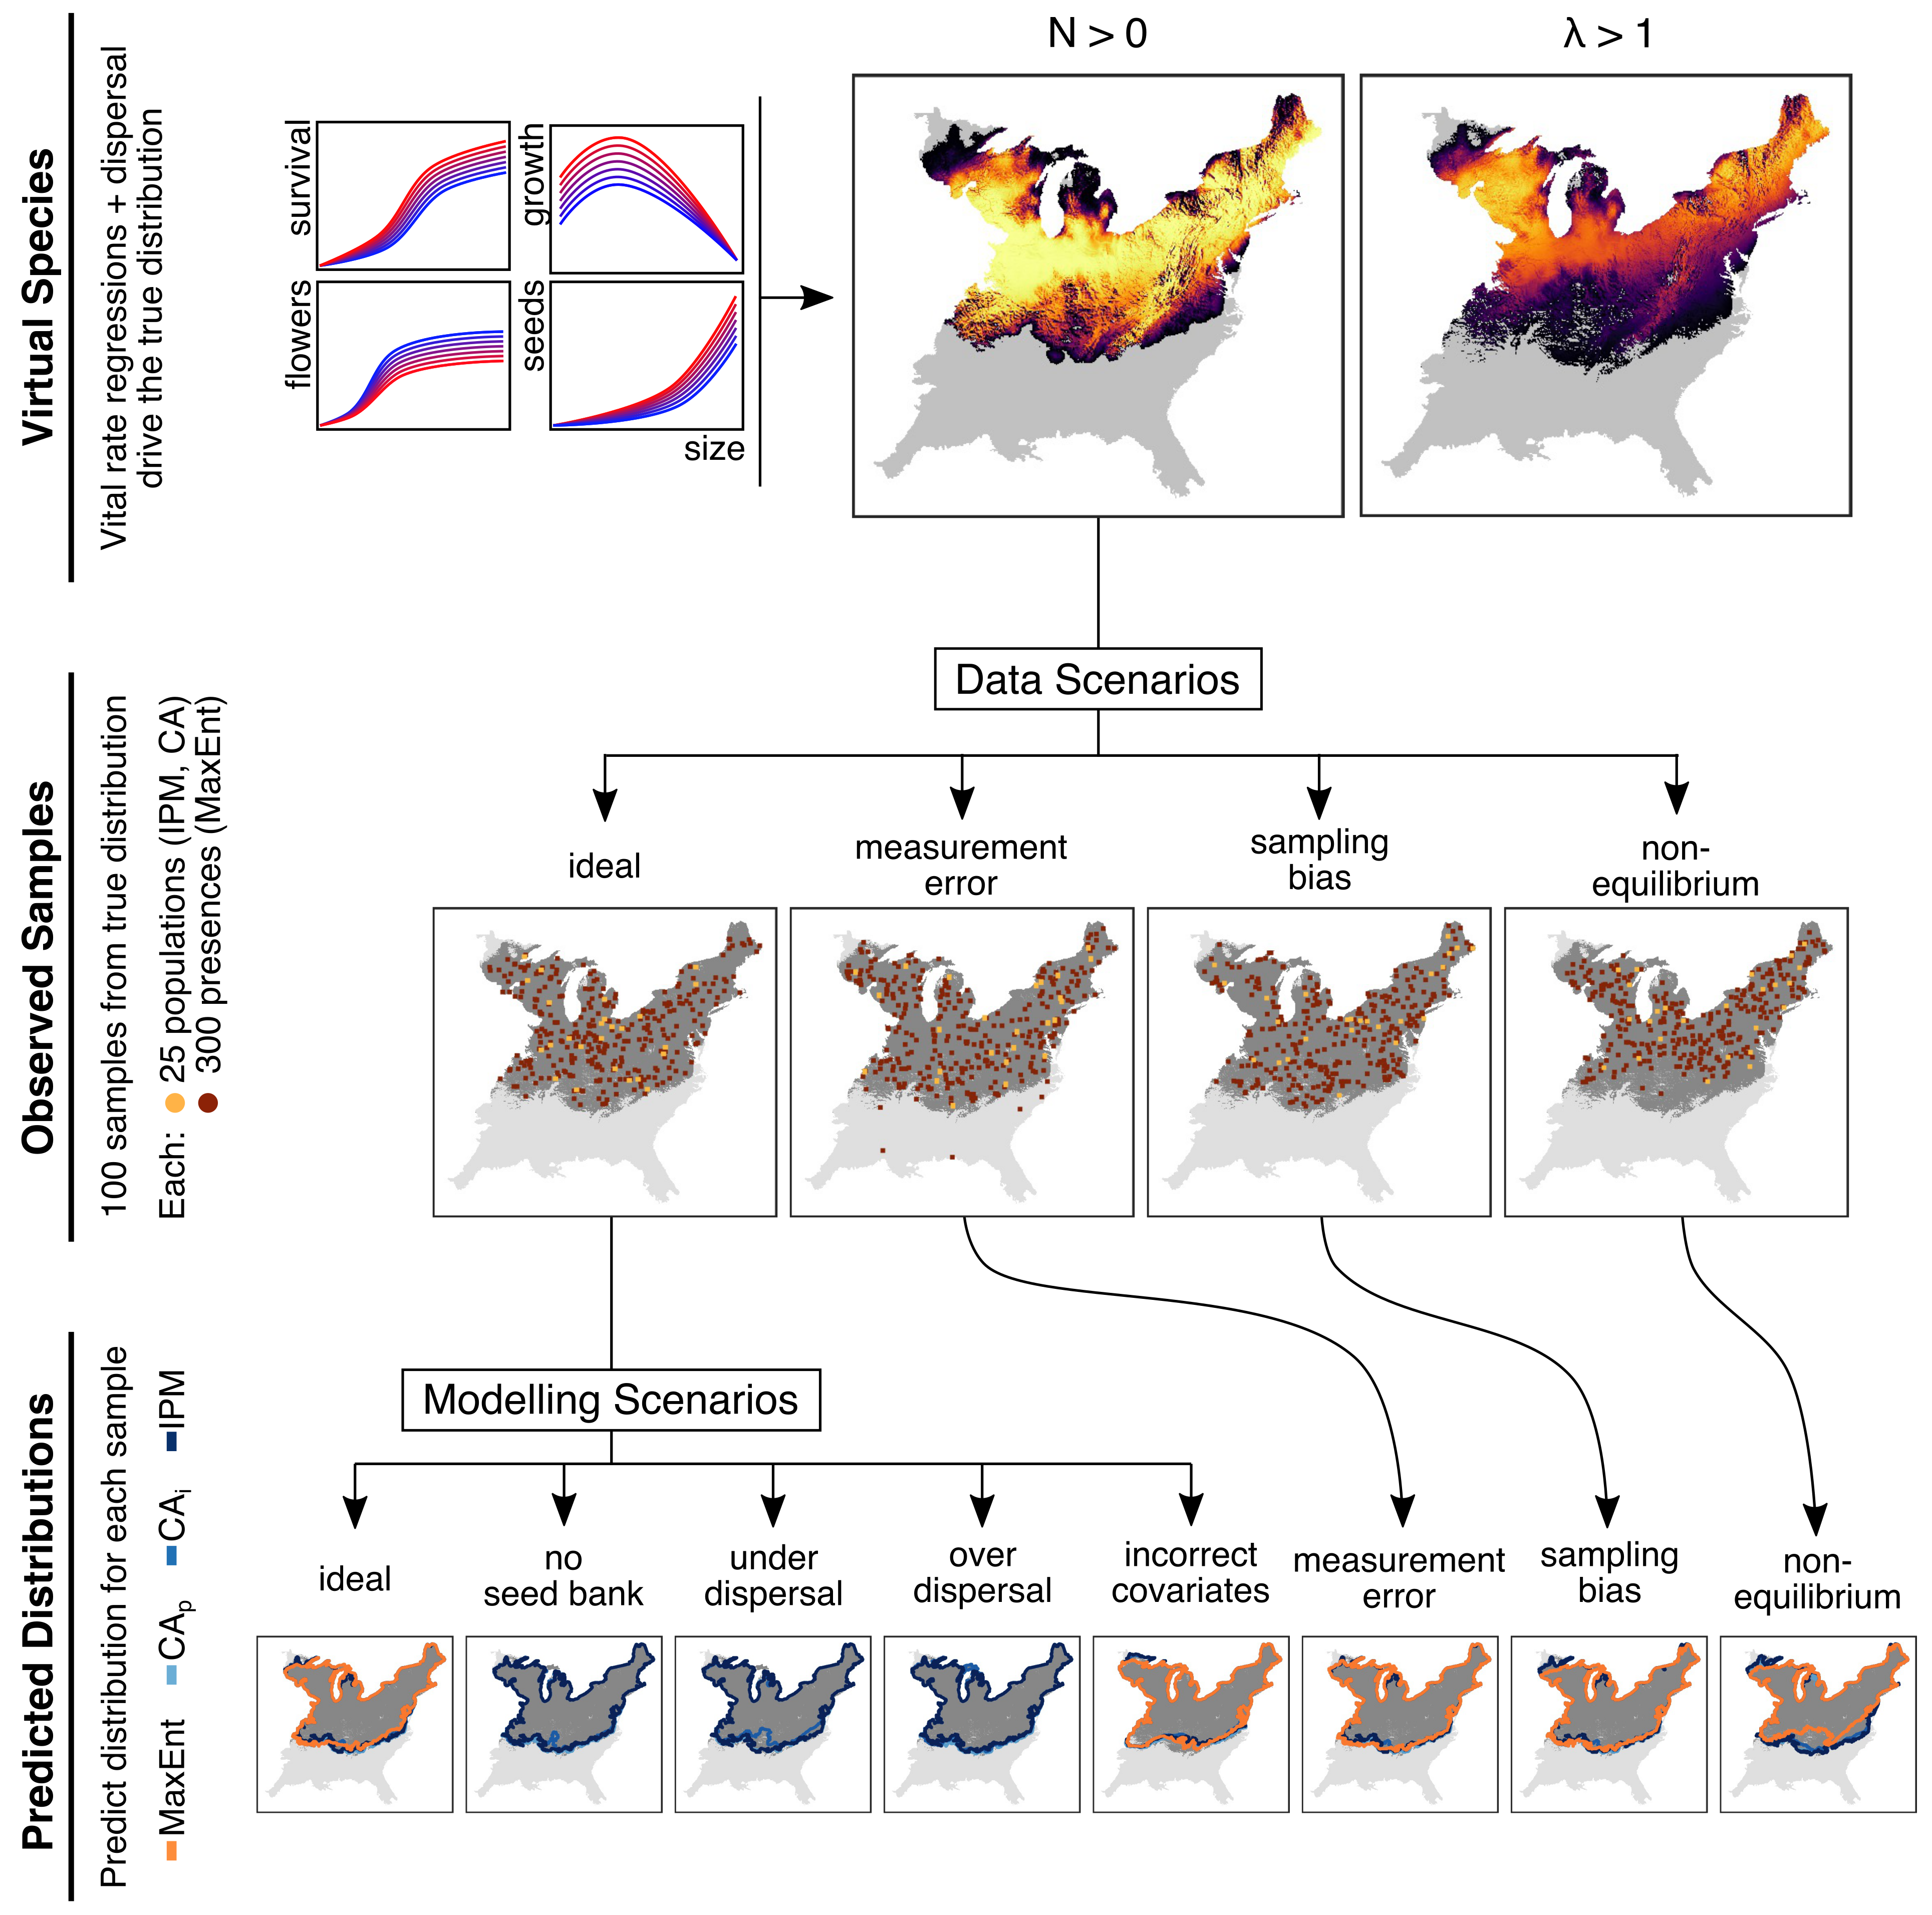
\includegraphics[width=5in]{../../figs/process_outline.png}
	\caption{\label{fig:outline} Simulation, sampling, and prediction process. Distributions were simulated for virtual species based on environmental effects on vital rates and demographic processes.}
\end{figure}
% General outline
We evaluated the performance of four species distribution models (SDMs) in predicting the ranges of two simulated species under a variety of data quality and modelling scenarios (Fig. 1), including one occurrence-based method (MaxEnt) and three process-based methods (Integral Projection Model: IPM; individual-level cellular automata: CA\textsubscript{i}; and population-level cellular automata: CA\textsubscript{p}). IPMs predict a deterministic intrinsic growth rate $\lambda$ in each cell of the landscape based on regressions of vital rates with environmental variables and individual sizes. In contrast, CA models are simulation-based and explicitly model spatio-temporal dynamics among cells. The CA\textsubscript{i} model simulates the growth, survival, and fecundity of individuals, while the CA\textsubscript{p} model uses population averages to summarize similar processes. See additional details for the process-based models in Appendix 1. 

\subsection{Virtual Species Simulation}
We simulated two virtual species in the eastern United States, based approximately on Japanese barberry (\emph{Berberis thunbergii}), an invasive shrub with bird-dispersed seeds, and garlic mustard (\emph{Alliaria petiolata}), an invasive biennial with seeds dispersed by non-volant animals and water. Both species have previously been the focus of process-based SDMs (CITE). To simulate each species, we defined relationships between environmental variables, individual size, and vital rates (Fig. \ref{fig:outline}, Appendix 1) on a gridded landscape spanning the Eastern Temperate Forest and Northern Forest ecozones within the United States ($\sim$5x5km resolution: 115,105 cells, CITE). Vital rates included annual individual growth, annual survival, flowering probability, seed production, and germination probability. For environmental covariates, we used the minimum temperature of the coldest month and the precipitation in May, following previous work (CITE PNAS, Chelsa). Based on these regressions, we calculated the intrinsic growth rate $\lambda$ in each cell following the methods used for IPMs, where each cell was treated as a population. Cells with $\lambda > 1$ were considered to be capable of containing persistent populations, constituting the first definition of the true distribution for each species.

To simulate populations, we initialized 10 random cells with 10 individuals, with individual sizes drawn from a uniform distribution constrained by the allowable range for each species. Then, we calculated the expected survival probability, growth rate, flowering probability, and seed production for each individual according to the vital rate regressions (Appendix 1). Then, we drew random values from the appropriate distributions for each vital rate for each individual, implemented short- and long-distance dispersal of seeds according to the dispersal mode of each species, and generated new individuals in each cell from germinating seeds. Populations in each cell were subject to density dependence through reduced seedling establishment (CITE) after the abundance exceeded a predetermined threshold. The populations were simulated through 300 years, at which point the distribution appeared stable, indicating that equilibrium had been reached. The cells with $N > 0$ in the final year thus constituted the second definition of the true distribution for each species.

\subsection{Sampling and Modelling Scenarios}
We evaluated four sampling scenarios: \emph{ideal} (year 300; uniform sampling probability among occupied cells), \emph{non-equilibrium} (year 100; uniform sampling probability among occupied cells), \emph{geographic bias} (year 300; sampling probability $\propto$ human and road density in occupied cells), and \emph{measurement error} (year 300; MaxEnt: 3\% of observations drawn from full landscape regardless of occupancy; process-based: error added to growth, seed production, and abundance observations). For each species, we generated 100 sets of sampled cells for each scenario. For MaxEnt, each sample consisted of 300 cells (CITE), while for the process-based SDMs, each sample consisted of 25 cells (CITE). For process-based models, a maximum of 1000 (CA\textsubscript{p}) or 100 (CA\textsubscript{i}, IPM) individuals were sampled from within each selected grid cell to reflect real-world logistical limitations (Appendix 1, https://github.com/Sz-Tim/sdmMethodComp). 

In addition, we assessed the effect of four scenarios of modeling misspecification: \emph{incorrect covariates}, \emph{no seed bank} (process-based only), \emph{over-estimated dispersal} (process-based only), \emph{under-estimated dispersal} (process-based only). Each of these misspecifications was implemented using the \emph{ideal} datasets. For \emph{incorrect covariates}, the SDMs were fit with correlated but more general climate variables (mean annual temperature, annual precipitation) rather than the more specific covariates used in the generative process and for all other scenarios (minimum temperature of the coldest month, precipitation in May).

For each scenario (Fig \ref{fig:outline}), the SDMs were parameterized using the corresponding sampled datasets. To select environmental covariates for each vital rate regression for each process-based SDMs, we compared all combinations of the climatic variables and their squares with the R package \emph{MuMIn}. For the CA\textsubscript{p} and CA\textsubscript{i} models, simulations were run for 300 years to generate predicted distributions. Using each definition of the true simulated ranges (i.e., $\lambda > 1$ and $N > 0$), we calculated the True Skill Statistic (TSS) for each of the 100 predicted distributions per scenario per SDM. We calculated TSS as $sensitivity + specificity - 1$, where $sensitivity$ is the proportion of true presences that are predicted correctly, and $specificity$ is the proportion of true absences that are predicted correctly, such that TSS ranges from $-1$ (all cells predicted incorrectly) to $1$ (all cells predicted correctly).






\section{Results}
\label{S:3}
% Talk results
% 1. Across all scenarios, IPM is best for lambda, CAi/p are best for N, with MaxEnt in the middle for both
% 2. Under ideal conditions, process-based outperform MaxEnt
% 3. For non-equilibrium distributions, process-based outperform MaxEnt
% 4. Process-based are much, much more sensitive to covariate choice -- implies sensitivity to regression accuracy
% 5. Dispersal is critical for CA models
% 6. Structural errors seem to have erratic effects
% 0. Process-based are better IF you are confident of the process, but MaxEnt is more robust to error and uncertainty

% Possible paragraphs:
% Rankings:
%	Ideal & mean(all scenarios): corresponding process-based is best on average
%	lambda = IPM, MxE, CA (avgs)
%	N = CA, MxE, IPM (avgs)
%	MaxEnt somewhat better for lambda
% Effect of data issues
%	Measurement error
% Effect of modelling issues
% Differences in output

% Rankings (overall, ideal)
All models performed well in recovering the true $\lambda$-based ($\lambda > 1$) and $N$-based distributions ($N>0$) for both species across all scenarios (all TSS medians $>$ 0.77), though no single model performed best universally (Fig. \ref{fig:TSSmn}). Across scenarios applicable to all four SDMs (Table \ref{table:ranks}), the IPM best predicted the $\lambda$-based distributions (mean rank: 1.5) and the CA models best predicted the $N$-based distributions (mean rank: CA\textsubscript{i}=1.6, CA\textsubscript{p}=1.9). MaxEnt was intermediate for both range boundaries on average (mean rank: $\lambda$-based=2.7, $N$-based=2.9)

\begin{table}
	\centering
	\captionsetup{width=.75\textwidth}
	\begin{tabular}{l c c c c}
		\hline \\[-3.5ex]
		\textbf{SDM} & \textbf{Best} & \textbf{Mean} & \textbf{Median} & \textbf{Worst}\\
		\hline 
		\hline \\[-2.5ex]
		\multicolumn{5}{l}{\textsc{True range: $\lambda > 1$}} \\
		CA\textsubscript{p} & 2 & 2.9 & 2.5 & 4\\
		CA\textsubscript{i} & 2 & 2.9 & 3 & 4\\
		IPM & 1 & 1.5 & 1 & 4\\
		MaxEnt & 1 & 2.7 & 2.5 & 4\\
		[.5ex]\hline \\[-2.5ex]
		\multicolumn{5}{l}{\textsc{True range: $N > 0$}} \\
		CA\textsubscript{p} & 1 & 1.9 & 2 & 3\\
		CA\textsubscript{i} & 1 & 1.6 & 1 & 4\\
		IPM & 3 & 3.6 & 4 & 4\\
		MaxEnt & 1 & 2.9 & 3 & 4\\
		[.5ex]\hline \\[-2ex]
	\end{tabular}
	\caption{\label{table:ranks}Summary of ranks across species and all scenarios applicable to all four SDMs. For each scenario and species, SDMs were ranked based on the median TSS.}
\end{table}

% Effect of data issues
For MaxEnt, TSS decreased when fit using samples from non-equilibrium populations, driven by smaller predicted ranges as indicated by a decrease in sensitivity (Fig. SXX:Sensitivity-Ideal) and a smaller increase in specificity (Fig. SXX:Specificity-Ideal). In contrast, non-equilibrium samples had minimal effect on TSS for the CA\textsubscript{p} model, with a modest improvement for the long-lived shrub in the IPM and CA\textsubscript{i} models driven by increases in sensitivity (Fig. SXX:Sensitivity-Ideal). Measurement error and sampling bias had negligible effects on the process-based models, and small to moderate effects on the performance of MaxEnt (Fig. \ref{fig:TSSmn}, Fig. SXX:Sensitivity-Ideal, Fig. SXX:Specificity-Ideal). 


\begin{figure}
	\centering\includegraphics[width=5in]{../../figs/fig_TSS_mn+CI.jpg}
	\caption{\label{fig:TSSmn} True skill statistic (TSS) mean and 95\% confidence intervals across 100 sampled datasets for each SDM and scenario, compared to true distributions defined by $\lambda > 1$ and $N > 0$. Scenarios include: no sampling or modeling issues (ideal), sampling issues (measurement error, sampling bias, non-equilibrium), and modeling issues (incorrect covariates, no seed bank, under dispersal, over dispersal).}
\end{figure}

\begin{figure}
	\centering\includegraphics[width=\linewidth]{../../figs/fig_TSSvIdeal.jpg}
	\caption{\label{fig:TSSvIdeal} Effect of scenario on median true skill statistic (TSS) relative to the '\emph{ideal}' scenario. Positive values indicate improved predictive ability, while negative values indicate decreased predictive ability.}
\end{figure}


% Effect of modelling issues
Modeling with incorrect covariates was universally problematic for model performance, though it had a greater impact on TSS in the shrub than the biennial species (Fig. \ref{fig:TSSvIdeal}). Incorrect covariates did not lead to systematic over-prediction or under-prediction, but rather a decrease in both sensitivity and specificity, particularly for the process-based models (Fig. SXX:Sensitivity-Ideal, Fig. SXX:Specificity-Ideal). Excluding the seed bank in the process-based models had minimal effect on TSS for the shrub, but variable effects on TSS for the biennial. Relative to ‘ideal’, all process-based models showed reduced sensitivity and increased specificity for the biennial, indicating a smaller predicted range. The IPM was generally more resistant to mischaracterized dispersal compared to the simulation-based CA\textsubscript{i} and CA\textsubscript{p} models. Underestimation of dispersal parameters led to decreased predicted ranges, and overestimation to increased predicted ranges relative to ‘ideal’. The effects were more extreme for the biennial than for the shrub.

% Process-based predictions (lambda, N, etc)
The process-based SDMs generate predictions for a number of biological quantities of interest. For instance, the IPM predicts $\lambda$ in each cell of the landscape. Discrepancies in predicted $\lambda$ values were biased downward in the northern portion of the study region (FIGURE 4), more strongly so for the shrub. Similarly, the CA models predict the abundance $N$ for each species. Discrepancies in predicted abundance from the CA\textsubscript{p} model showed a spatial banding of upward bias at the range margins for both species (FIGURE 4). Immediately interior to the range margin, the CA\textsubscript{p} and CA\textsubscript{i} model showed upward bias for the shrub (FIGURE 4). 




\section{Discussion}
\label{S:4}

% Talk Discussion
% 1. Across all scenarios, IPM is best for lambda, CAi/p are best for N, with MaxEnt in the middle for both
% 2. Under ideal conditions, process-based outperform MaxEnt
% 3. For non-equilibrium distributions, process-based outperform MaxEnt
% 4. Process-based are much, much more sensitive to covariate choice -- implies sensitivity to regression accuracy
% 5. Dispersal is critical for CA models
% 6. Structural errors seem to have erratic effects
% 0. Process-based are better IF you are confident of the process, but MaxEnt is more robust to error and uncertainty

% Overview
This is the first paragraph summarizing some general stuff. The process-based SDMs provide a lot more information, and they do, in fact, perform a bit better on average. They are less impacted by samples from non-equilibrium populations, so that is in line with expectations. However, they are more susceptible to mismatches in the covariates than MaxEnt, and the structural errors in the models don't necessarily have predictable effects. 

% Process-based > MaxEnt under ideal conditions, and especially non-equilibrium distributions
Expand on the summary, bringing in past work on non-equilibrium distributions. Since process-based models aim to describe the biological processes that ultimately produce an emergent distribution, it really doesn't matter whether the samples are from a non-equilibrium species as long as the populations contain a sufficiently broad span of ages or sizes. This points to the fact that in parameterizing process-based models, care should be taken to select populations with a mix of ages or sizes rather from a range of environmental conditions than focusing on the geographic distribution per se, in essence capturing more of the parameter space. Thus, for non-equilibrium species, a well-described process-based SDM should do better than an occurrence-based model.
.
% However, process-based are highly sensitive
%	- covariate choice: even highly correlated covariates lead to dramatically decreased ability
%	- dispersal: critical for CA models
% 	- structural errors seem to have erratic effects
However, process-based models appear to be sensitive to several parts of the modelling process. First, they are much more sensitive to covariate choice, and by generalization, to the alignment of the modelled relationship between vital rates and the environment with reality. The flexible structure of MaxEnt, perhaps along with the top-down perspective, makes it much less influenced by errors in the covariates. Even with covariates that are highly correlated with the true covariates, there is still a large decrease in predictive ability for the process-based models. 

% So: Why or when to use each?
%	- MaxEnt is probably best for most species: fairly robust, already know about non-equilibrium, etc
%		- But what about climate change? Isn't everything at disequilibrium now? Shit...
%	- is it justifiable to draw conclusions about long-lived vs short-lived species? 
%		- We should have done these simulations with everything else identical but that (climatic preferences, etc)
%		- redo each with just the lifespan changed? But that will probably just make it more complicated....
% Range boundaries: What is each SDM predicting?


% Range boundaries
Range boundaries can be defined in several ways. For the true distribution of each species, we use two definitions: abundance-based (cells with $N > 0$) and $\lambda$-based (cells with $\lambda > 1$). The process-based SDMs compared here each predict a specific type of range boundary. IPMs predict $\lambda$ in each cell of the landscape, while the simulation-based CA models predict abundance. For MaxEnt, the range boundary definition is less explicit. The geo-located presences used as input imply an abundance-based range, but predicted distributions are frequently constrained by a data-based threshold (e.g., relative suitability values that encapsulate 95\% of the observed data) to exclude both erroneous data and sink populations, which implies an effort to predict a $\lambda$-based range. Generally, process-based SDMs explicitly predict one type of range or another, while occurrence-based SDMs may be rather ambiguous. There may or may not be a big difference between the two range definitions, but it will depend on the species. For example, the magnitude of the difference should vary with the number or distribution of marginal cells (lots of marginal cells mean large areas with middling occupancy probabilities), the typical annual stochasticity in the population abundances (more stochasticity means more discrepancies are likely), and dispersal limitation (high dispersal or a long introduction history means fewer areas that have not been reached, but also possibly a larger proportion of sink populations). 



\section{Acknowledgments}
This project was funding through National Science Foundation award IIS-1717368. 


\section{Bibliography}

\end{document}
